\documentclass{article}
\usepackage{amsmath}
\usepackage{hyperref}
\title{CS 250 Course Study Guide}
\author{Sarmistha Sarna Gomasta, Kyla Levin, Alexander Yeung}
\date{Fall 2023}

\usepackage[letterpaper, portrait, margin=1in]{geometry}
\usepackage{graphicx}
\usepackage{enumitem}
\usepackage{ulem}
\usepackage{amssymb}
\usepackage{amsmath}
\usepackage{tikz}
\usepackage{url}
\usepackage{color}   %May be necessary if you want to color links
\usepackage{hyperref}
\hypersetup{
    colorlinks=true, %set true if you want colored links
    linktoc=all,     %set to all if you want both sections and subsections linked
    linkcolor=black,  %choose some color if you want links to stand out
}


\begin{document}

\maketitle
\begin{center}
    \textbf{Please Fill Out Our Feedback Form: \href{https://forms.gle/1ieupiHHHSuTEjXe9}{https://forms.gle/1ieupiHHHSuTEjXe9}}
\end{center}
\section*{Notes on Intended Use:}
We hope you find this study guide useful, however, we would like to make a few notes on its intended use. 
\begin{center}
    \begin{enumerate}
        \item This study guide is not intended to be exhaustive. Its intended purpose is for you to ascertain whether or not you have a basic understanding of each topic. \textit{Please use other resources (lecture notes, past exams, etc.) to study for the final.}
        \item This resource was made by graduate students as a learning supplement and may not perfectly reflect exam-level difficulty.
        \item We advise you to use this to first to gauge your basic understanding of a topic before filling in any gaps in your knowledge with other materials to improve practice exam performance.
    \end{enumerate}
    
\end{center}

\tableofcontents
\newpage



\section*{Chapter 1: Sets and Predicate Logic}
\addcontentsline{toc}{section}{Chapter 1: Sets and Predicate Logic}
\subsection*{Q1.1}
\addcontentsline{toc}{subsection}{Q1.1}
Solve the following syllogism. Report the answer as a logical implication, as well as a naturally-spoken English sentence.
\begin{itemize}
    \item The only foods that my doctor recommends are ones that aren't very sweet.
    \item Nothing that agrees with me is good for dinner.
    \item Cake is always very sweet.
    \item My doctor recommends all foods that are good for dinner.
\end{itemize}
\newpage
% \subsection*{Q1.1 Answer}
% \addcontentsline{toc}{subsection}{Q1.1 Answer}
% We will use the following variables: $D=\text{doctor recommends it},S=\text{sweet},A=\text{agrees with me},G=\text{good for dinner}$
% \begin{itemize}
%     \item This can be read as "If my doctor recommends it, then it's not very sweet." $D\rightarrow \neg S$
%     \item This can be read as "There is nothing such that if it agrees with me, then it's good for dinner." $A\rightarrow G$
%     \item This can be read as "If it's cake, then it's very sweet." $C\rightarrow S$
%     \item This can be read as "If it's good for dinner, then my doctor recommends it." $G\rightarrow D$
% \end{itemize}
% $C\rightarrow S\rightarrow \neg D\rightarrow\neg G$
% \\ Transitively, $C\rightarrow\neg G$
% \\ In English, "If it's cake, then it's not good for dinner." Or, more naturally, "Cake is not good for dinner."
% \newpage
\addcontentsline{toc}{subsection}{Q1.2}
\subsection*{Q1.2}
\begin{enumerate}[label=\alph*.]
    \item What values of $a$ and $b$ make the following statement true? Prove using a truth table.
    $$(a \lor \neg b) \land (b \land \neg a)$$
    \item What values of $a$, $b$, and $c$ make the following statement true? Prove without using a truth table.
    $$(a \lor \neg b) \land (b \land \neg a)\rightarrow (\neg c\land(a \lor b))$$
\end{enumerate}
\newpage
% \subsection*{Q1.2 Answer}
% \addcontentsline{toc}{subsection}{Q1.2 Answer}
% \begin{enumerate}[label=\alph*.]
%     \item What values of $a$ and $b$ make the following statement true? Prove using a truth table.
%     $$(a \lor \neg b) \land (b \land \neg a)$$
%     \begin{tabular}{|c|c|c|c|c|c|c|}
%      \hline
%      $a$ & $b$ & $\neg a$ & $\neg b$ & $(a\lor \neg b)$ & $(b\land\neg a)$ & $(a\lor \neg b)\land(b\land\neg a)$ \\ 
%      \hline
%      T & T & F & F & T & F & F \\  
%      T & F & F & T & T & F & F \\
%      F & T & T & F & F & T & F \\  
%      F & F & T & T & T & F & F \\
%      \hline
%     \end{tabular}
%     \\ To fill in the truth table, begin with the primitive values $a$ and $b$ in the leftmost columns. From there, use those values to fill in the successive $\neg a$ and $\neg b$ values in the next two columns. Continue rightways, adding columns with increasingly complex expressions using the truth values from the simpler columns until you have constructed the final expression.
%     \\ As a reminder, for the binary operator "OR" ($\lor$), \textit{at least one} of the input needs to be true. For the binary operator "AND" ($\land$), \textit{both} of the input need to be true. And the unary operator "NOT" ($\neg$) will flip the truth value of its input.
%     \\ As seen in the final column of the truth table, there is no combination of $a$ and $b$ values that make $(a\lor \neg b)\land(b\land\neg a)$ true.
%     \item What values of $a$, $b$, and $c$ make the following statement true? Prove without using a truth table.
%     $$(a \lor \neg b) \land (b \land \neg a)\rightarrow (\neg c\land(a\lor b))$$
%     \\ All possible values of $a$, $b$, and $c$ will make this statement true. We know from part (a) that the antecedent of the implication step is always false. There are no $a$ and $b$ values that make it true. Therefore, there is no value that the consequent could have to make the whole implication evaluate to true. If the consequent is true, then $F\rightarrow T$ evaluates to true. If the consequent is false, then $F\rightarrow F$ still evaluates to true. 
% \end{enumerate}
% \newpage
\subsection*{Q1.3}
\addcontentsline{toc}{subsection}{Q1.3}
Complete a deductive sequence proof based on the following propositions:
\begin{enumerate}
    \item $\lnot p \land q$
    \item $r \rightarrow p$
    \item $\lnot r \rightarrow s$
    \item $s \rightarrow t$
\end{enumerate}
Your answer should either be a conjunction of all of the variables p,q,r,s,t which enumerates their
truth values, or you may explicitly state the truth value of each variable.
\newpage
% \subsection*{Q1.3 Answer}
% \addcontentsline{toc}{subsection}{Q1.3 Answer}
% \begin{enumerate}
%     \item Assume $\lnot p$
%     \item q (Premise 1, right separation)
%     \item $\lnot p \rightarrow \lnot r$ (Contrapositive of Premise 2)
%     \item $\lnot r$ (Modus Ponens of Line 3)
%     \item $s$ (Modus Ponens of Premise 3)
%     \item $t$ (Modus Ponens of Premise 4)
% \end{enumerate}
% Then our final solution is $\lnot p \land q \land \lnot r \land s \land t$
% \newpage

\subsection*{Q1.4}
\addcontentsline{toc}{subsection}{Q1.4}
Prove by contradiction that the sum of a rational number and an irrational number is irrational. Recall that a rational number is one
which can be expressed as the quotient of two integers. An irrational number is one which cannot be represented as the quotient of two integers.
You may assume that the operations addition, subtraction, and multiplication on rationals are well-defined. In other words, the sum, difference, or
product of two rationals is always rational.
\newpage
% \subsection*{Q1.4 Answer}
% \addcontentsline{toc}{subsection}{Q1.4 Answer}
% Assume to the contrary, $\exists s$ such that $s = r + i$ where $r \in \mathbb{Q}$, the rational numbers, and $i \notin \mathbb{Q}$, or i is irrational.
% Well, then $i = s - r$. But we know that the difference between two rational numbers is always rational. Then i must be a rational number. But this is a contradiction
% because we assumed i to be irrational! 
% \newpage

\subsection*{Q1.5}
\addcontentsline{toc}{subsection}{Q1.5}
Prove that if $n$ is divisible by 6, then $n+10$ is not divisible by 6.
\newpage
% \subsection*{Q1.5 Answer}
% \addcontentsline{toc}{subsection}{Q1.5 Answer}
% First, we must assume the antecedent to prove the consequent, so assume that $n$ is divisible by 6.
% \\ Now, for the sake of contradiction, assume that $n+10$ \textit{is} divisible by 6. If this is the case, then both $6|n$ and $6|(n+10)$ are true, therefore $6|(n+10-n)$
% \\ If you require proof of this property, it can be observed below:
% \begin{enumerate}[label=]
% \item Claim: If $a|b$ and $a|c$, then $a|(b-c)$
% \\ If $a|b$, then by the definition of divisibility, $\exists n\in\mathbb{Z}:an=b$
% \\ If $a|c$, then by the definition of divisibility, $\exists m\in\mathbb{Z}:am=c$
% \\ Subtracting one equation from the other: $an-am=a(n-m)=b-c$
% \\ Since $n-m\in\mathbb{Z}$, then by definition of divisibility, $a|(b-c)$
% \end{enumerate}
% Back to the original proof: If $6|(n+10-n)$, then this simplifies to $6|10$, however, this is not true. 6 does not divide 10, therefore we have a contradiction.
% \newpage

\subsection*{Additional Resources for Sets and Predicate Logic}
\addcontentsline{toc}{subsection}{Additional Resources}
\begin{enumerate}
    \item \href{https://www.youtube.com/watch?v=A2k3ulOJ3u4}{Translating Statements to Propositional Logic} 
    \item \href{https://www.youtube.com/watch?v=A3Ffwsnad0k&list=PLl-gb0E4MII28GykmtuBXNUNoej-vY5Rz}{Excellent Discrete Math Playlist}
    \item \href{https://www.youtube.com/watch?v=6o1kLNEE-d4&list=PLF_J2w5w0Z3E7jZGz-23P6WrKxokXBkHC}{Playlist Containing Many Worked Out Deductive Proofs}
    \item \href{https://www.youtube.com/watch?v=CpW0ZJ7i0oc}{MIT Video of Proof by Contradiction}
    \item \href{https://www.youtube.com/watch?v=0YqZIHFmVzg}{Proof by Contrapositive Intro}
    \item \href{https://www.youtube.com/watch?v=8DW0K3mnc-0}{Rules of Inference Video}
\end{enumerate}
\newpage

\section*{Chapter 2: Quantifiers and Relations}
\addcontentsline{toc}{section}{Chapter 2: Quantifiers and Relations}

\subsection*{Q2.1}
\addcontentsline{toc}{subsection}{Q2.1}
Consider the set $A=\mathbb{N}$
\\ Identify whether the following relations are reflexive, antireflexive, symmetric, antisymmetric, or transitive.
\begin{itemize}
    \item $x$ relates to $y$ if and only if $x=2y$ 
    \item $x$ relates to $y$ if and only if $x\%2=y\%2$
\end{itemize}
\newpage
% \subsection*{Q2.1 Answer}
% \addcontentsline{toc}{subsection}{Q2.1 Answer}
% \begin{itemize}
%     \item $x$ relates to $y$ if and only if $x=2y$
%     \\ This is not reflexive, because for most numbers, $x\neq 2x$. However, it is also not antireflexive, since $x=2x$ is true for $x=0$. It is not symmetric, since if $x=2y$, then $y\neq2x$. The only case when this is true is for $x=y=0$, when $x$ and $y$ are the same. Therefore, this relation is antisymmetric. It is not transitive, since if $x=2y$ and $y=2x$, then $x=4z$, which is not always equal to $2z$.
%     \item $x$ relates to $y$ if and only if $x\%2=y\%2$
%     \\ This is reflexive, since $x\%2=x\%2$ for all $x$. Because it is reflexive, it cannot be antireflexive. It is symmetric, since if $x\%2=y\%2$, then   $y\%2=x\%2$. It is not antisymmetric, since this can be true of different $x$ and $y$ values. It is transitive, since if $x\%2=y\%2$ and $y\%2=z\%2$, then $x\%2=z\%2$.
% \end{itemize}
% \newpage

\subsection*{Q2.2}
\addcontentsline{toc}{subsection}{Q2.2}
Let \( A, B, C, D \) be nonempty sets.
\begin{enumerate}
    \item[a)] Prove that \( A \times B \subseteq C \times D \) if and only if \( A \subseteq C \) and \( B \subseteq D \).
    \item[b)] What happens to the result in part (a) if any of the sets \( A, B, C, D \) is empty?
\end{enumerate}
\newpage
% \subsection*{Q2.2 Answer}
% \addcontentsline{toc}{subsection}{Q2.2 Answer}
% \begin{enumerate}
%     \item[(a)] Assume that \( A \times B \subseteq C \times D \) and let \( a \in A \) and \( b \in B \). Then \( (a, b) \in A \times B \), and since \( A \times B \subseteq C \times D \) we have \( (a, b) \in C \times D \). But \( (a, b) \in C \times D \) implies \( a \in C \) and \( b \in D \). Hence, \( a \in A \) implies \( a \in C \), so \( A \subseteq C \), and \( b \in B \) implies \( b \in D \), so \( B \subseteq D \).
%     Conversely, suppose that \( A \subseteq C \) and \( B \subseteq D \), and that \( (x, y) \in A \times B \). Then \( x \in A \) and \( y \in B \) implies \( x \in C \) (since \( A \subseteq C \)) and \( y \in D \) (since \( B \subseteq D \)) implies \( (x, y) \in C \times D \). Consequently, \( A \times B \subseteq C \times D \).
%     \item[(b)] If any of the sets \( A, B, C, D \) is empty we still find that
%     \[
%     \{ (A \subseteq C) \land (B \subseteq D) \} \Rightarrow \{ A \times B \subseteq C \times D \}.
%     \]
%     However, the converse need not hold. For example, let \( A = \emptyset \), \( B = \{1, 2\} \), \( C = \{1, 2\} \) and \( D = \{1\} \). Then \( A \times B = \emptyset \) --- if not, there exists an ordered pair \( (x, y) \) in \( A \times B \), and this means that the empty set \( A \) contains an element \( x \). And so \( A \times B = \emptyset \subseteq C \times D \) --- but \( B = \{1, 2\} \not\subseteq \{1\} = D \).
% \end{enumerate}
% \newpage

\subsection*{Q2.3}
\addcontentsline{toc}{subsection}{Q2.3}
 Determine whether or not each of the following relations is a function. If a relation is a function, find its range.

\begin{enumerate}
    \item[a)] \( \{ (x, y) \mid x, y \in \mathbb{Z}, y = x^2 + 7 \} \), a relation from \(\mathbb{Z}\) to \(\mathbb{Z}\)
    \item[b)] \( \{ (x, y) \mid x, y \in \mathbb{R}, y^2 = x \} \), a relation from \(\mathbb{R}\) to \(\mathbb{R}\)
    \item[c)] \( \{ (x, y) \mid x, y \in \mathbb{R}, y = 3x + 1 \} \), a relation from \(\mathbb{R}\) to \(\mathbb{R}\)
    \item[d)] \( \{ (x, y) \mid x, y \in \mathbb{Q}, x^2 + y^2 = 1 \} \), a relation from \(\mathbb{Q}\) to \(\mathbb{Q}\)
    \item[e)] \( \mathcal{R} \) is a relation from \( A \) to \( B \) where \( |A| = 5 \), \( |B| = 6 \), and \( |\mathcal{R}| = 6 \).
\end{enumerate}
\newpage
% \subsection*{Q2.3 Answer}
% \addcontentsline{toc}{subsection}{Q2.3 Answer}
% \begin{enumerate}
%     \item[(a)] Function: Range = \{7, 8, 11, 16, 23, \ldots\}
%     \item[(b)] Relation, not a function. For example, both (4,2) and (4, -2) are in the relation.
%     \item[(c)] Function: Range = the set of all real numbers.
%     \item[(d)] Relation, not a function. Both (0,1) and (0, -1) are in the relation.
%     \item[(e)] Since \( |\mathcal{R}| > 5 \), \( \mathcal{R} \) cannot be a function.
% \end{enumerate}
% \newpage

\subsection*{Q2.4}
\addcontentsline{toc}{subsection}{Q2.4}
Determine whether each of the following statements is true or false. If it is true, give a short proof. If it is false, give an example.
\begin{enumerate}[label=\alph*.]
    \item If \( x \in A \) and \( A \in B \) (not a typo), then \( x \in B \).
    \item If \( A \subseteq B \) and \( B \in C \), then \( A \in C \).
    \item If \( A \subseteq B \) and \( B \subseteq C \), then \( A \subseteq C \).
    \item If \( A \not\subset B \) and \( B \not\subseteq C \), then \( A \not\subseteq C \).
    \item If \( x \in A \) and \( A \not\subseteq B \), then \( x \in B \).
    \item If \( A \subseteq B \) and \( x \notin B \), then \( x \notin A \).
\end{enumerate}
\newpage
% \subsection*{Q2.4 Answer}
% \addcontentsline{toc}{subsection}{Q2.4 Answer}
% \begin{enumerate}[label=\alph*.]
% \item \textbf{False.} Let \( A = \{1, 2\} \) and \( B = \{ \{1, 2\}, \{3\}\} \). Now, consider $x=2$. The premises are met since \( 2 \in \{1, 2\} \) and \( \{1, 2\} \in \{ \{1, 2\},\{3\}\} \). However, \( 2 \notin \{\{1, 2\},\{3\}\} \).
% \item \textbf{False.} Let \( A = \{2\} \), \( B = \{0, 2\} \), and \( C = \{\{1\}, \{0, 2\}, \{2, 3\}\} \). The premises are met since $A\subseteq B$ and $B\in C$. However, \( A \notin C \).
% \item \textbf{True.} Assume \( A \subseteq B \) and \( B \subseteq C \). Let there be some $x$ such that \( x \in A \). Because $A\subseteq B$, this implies that \( x \in B \). Because $B\subseteq C$, this implies that \( x \in C \). Therefore, for any arbitrary element $x\in A$, we can conclude that $x\in C$ and therefore \( A \subseteq C \).
% \item \textbf{False.} $A$ being dissimilar from $B$ and $B$ being dissimilar from $C$ does not imply that $A$ and $C$ are dissimilar. Let \( A = \{1, 2\} \), \( B = \{0, 6, 8\} \), and \( C = \{0, 1, 2, 6, 9\} \). Neither $A\subseteq B$ or $B\subseteq C$, however, \( A \subseteq C \).
% \item \textbf{False.} Let \( A = \{3, 5, 7\} \) and \( B = \{3, 4, 6\} \). Now, let $x=5$. \( 5 \in A \) and \( A \nsubseteq B \). However, \( 5 \notin B \).
% \item \textbf{True.} Assume \( A \subseteq B \) and let there be some $x$ such that \( x \notin B \). For the sake of contradiction, assume \( x \in A \). Then because $A\subseteq B$, \( x \in B \), which is a contradiction as \( x \notin B \). Therefore, \( x \notin A \).
% \end{enumerate}
% \newpage

\subsection*{Q2.5}
\addcontentsline{toc}{subsection}{Q2.5}
Suppose you have sets $A=\{3,5,7,11,13,17\}$ and $B=\{0,1,2,3,5,8,13\}$ and some function $f:A\rightarrow B$.
\begin{enumerate}[label=\alph*.]
\item How many one-to-one functions $f$ are possible? Give one example.
\item How many onto functions $f$ are possible? Give one example.
\end{enumerate}
\newpage
% \subsection*{Q2.5 Answer}
% \addcontentsline{toc}{subsection}{Q2.5 Answer}
% \begin{enumerate}[label=\alph*.]
% \item A "one-to-one" function is one where each input leads to a distinct output. So any example where no two elements of $A$ lead to the same element of $B$ is a valid answer. Think of this as selecting an output for each input. For the first input, $3\in A$, there are 7 possible outputs in $B$. Since the outputs must be distinct in a one-to-one function, there are 6 possible outputs for the next element of $A$, 5 for the next, and so on and so forth. So for 6 possible inputs, there are $7\cdot6\cdot5\cdot 4\cdot3\cdot2=5,040$ possible one-to-one functions. For the simplest example, $f=\{(3,0),(5,1),(7,2),(11,3),(13,5),(17,8)\}$
% \item An "onto" function is one where every possible output has a corresponding input. This is, however, not possible since there are more possible outputs than there are possible inputs. To achieve every possible output, at least two inputs would have to lead to the same output. This can also not be the case, since this would not be a function. So no onto functions $f$ are possible.
% \end{enumerate}
% \newpage

% \begin{comment}
% \subsection*{Q2.6}
% \addcontentsline{toc}{subsection}{*Q2.5}
% \begin{enumerate}
%    \item[a)] Let \( a \in \mathbb{R}^+ \) where \( a \geq 1 \). Prove that (i) \( \left\lfloor \frac{a}{a} \right\rfloor = 1 \); and (ii) \( \left\lfloor \frac{1}{a}\right\rfloor = 0 \).
%    \item[b)] If \( a \in \mathbb{R}^+ \) and \( 0 < a < 1 \), which result(s) in part (a) is (are) true?
% \end{enumerate}
% \newpage
% \subsection*{Q2.6 Answer}
% \addcontentsline{toc}{subsection}{*Q2.5 Answer}
% \begin{enumerate}
%     \item[a)] Proof (i): If \( a \in \mathbb{Z}^+ \), then \( \lfloor a \rfloor = a \) and \( \lfloor \frac{a}{a} \rfloor = 1 \). If \( a \notin \mathbb{Z}^+ \), write \( a = n + c \), where \( n \in \mathbb{Z}^+ \) and \( 0 < c < 1 \). Then \( \lfloor \frac{a}{a} \rfloor = \lfloor (n + 1)/(n + c) \rfloor = 1 + \lfloor (1 - c)/(n + c) \rfloor \), where \( 0 < (1 - c)/(n + c) < 1 \). Hence \( \lfloor \frac{a}{a} \rfloor = 1 + \lfloor (1 - c)/(n + c) \rfloor = 1 \).
% 	Proof (ii): For \( a \in \mathbb{Z}^+ \), \( \lfloor a \rfloor = a \) and \( \lfloor \frac{1}{a} \rfloor = 0 \) and \( \lfloor \frac{1}{a} \rfloor = \lfloor 1 \rfloor = 1 \). When \( a \notin \mathbb{Z}^+ \), let \( a = n + c \), where \( n \in \mathbb{Z}^+ \) and \( 0 < c < 1 \). Then \( \lfloor \frac{1}{a} \rfloor = \lfloor 1/(n + c) \rfloor = 1 - \lfloor c/(n + c) \rfloor \), where \( 0 < c/(n + c) < 1 \). Consequently \( \lfloor \frac{1}{a} \rfloor = 1 - \lfloor c/(n + c) \rfloor = 1 \).
%     \item[b)] Consider \( a = 0.1 \). Then the following:
% \begin{enumerate}
%     \item[i)] \( \lfloor \frac{a}{a} \rfloor = \lfloor 0.1/0.1 \rfloor = \lfloor 1 \rfloor = 1 \) is equal to 1
%     \item[ii)] \( \lfloor \frac{1}{a} \rfloor = \lfloor 1/0.1 \rfloor = 0 \) not equal to 1
% \end{enumerate}
% In fact (ii) is false for all \( 0 < a < 1 \), since \( \lfloor \frac{1}{a} \rfloor = 0 \) for all such values of \( a \). In the case of (i), when \( 0 < a \leq 0.5 \), it follows that \( \lfloor \frac{a}{a} \rfloor \geq 2 \) and \( \lfloor \frac{1}{a} \rfloor \geq 2 \) not equal to \( f \). However, for \( 0.5 < a < 1 \), \( \lfloor \frac{a}{a} \rfloor = \frac{1}{a} \) where \( 1 < \frac{1}{a} < 2 \), and so \( \lfloor \frac{a}{a} \rfloor = 1 \) for \( 0.5 < a < 1 \).
% \end{enumerate}
% \newpage

\subsection*{Additional Resources for Quantifiers and Relations}
\addcontentsline{toc}{subsection}{Additional Resources}
\begin{enumerate}
    \item \href{https://www.youtube.com/watch?v=tyDKR4FG3Yw&list=PLDDGPdw7e6Ag1EIznZ-m-qXu4XX3A0cIz}{Set Theory Playlist}
    \item \href{https://www.youtube.com/watch?v=ZgcTX16borA}{Equivalence Relations and Equivalence Classes Explained}
    \item \href{https://www.youtube.com/watch?v=bZred_Ksz2k&t=6s}{Bijective, Injective, Surjective Explained}
    \item \href{https://www.youtube.com/watch?v=GJpezCUMOxA}{Existential and Universal Quantifiers Explained}
    \item \href{https://www.youtube.com/watch?v=q1rKFGSiZE8}{Negating Quantifiers}
    \item \href{https://www.youtube.com/watch?v=jLVKV5LJjaw}{Negating Multiple Quantifiers}
    \item \href{https://www.youtube.com/watch?v=6fwJj14O_TM}{Reflexive, Symmetric, Transitive}
\end{enumerate}
\newpage

\section*{Chapter 3: Number Theory}
\addcontentsline{toc}{section}{Chapter 3: Number Theory}

\subsection*{Q3.1}
\addcontentsline{toc}{subsection}{Q3.1}
Prove that for some relatively prime $a$ and $n$, multiplying all numbers in the set $\{1,2,...,n-2,n-1\}$ by $a$ will output a permutation of $\{1,2,...,n-2,n-1\}$.
\\ Hint: There are two parts to this proof---existence and uniqueness. To show that multiplication by $a$ permutes the elements of the set, you must show that the multiplication always produces an element in the set (existence) and you must show that that element will never be repeatedly produced via multiplication by $a$ (uniqueness). Consider how these relate to modular arithmetic and modular inverses.
\newpage
% \subsection*{Q3.1 Answer}
% \addcontentsline{toc}{subsection}{Q3.1 Answer}
% As stated in the hint, we must show both the existence and uniqueness of the elements from the set when multiplied by $a$.
% \\ First, to prove existence, we will prove that for some relatively prime $a$ and $n$, and for some elements $b,c\in \{1,2,...,n-2,n-1\}$,  $ab=c$ (mod $n$), unless $b=0$. This is equivalent to saying that "If $ab=0$ (mod $n$), then $b=0$ (mod $n$)". Since $a$ and $n$ are relatively prime, $a$ has an inverse in mod $n$. Multiply both sides by $a^{-1}$ (mod $n$) to get $aba^{-1}=0(a^{-1})$ (mod $n$). $aa^{-1}$ will cancel out to 1, showing that $b=0$ (mod $n$).
% \\ Next, to prove uniqueness, we will show that for some relatively prime $a$ and $n$, if $ab=ac$ (mod $n$), then $b=c$. Once again, because $a$ and $n$ are relatively prime, we know $a$ must have some inverse $a^{-1}$ (mod $n$). Multiplying both sides by $a^{-1}$ gives $aba^{-1}=aca^{-1}$ (mod $n$), leaving $b=c$ (mod $n$).
% \\ Putting the two pieces together, we know that multiplying any element of $\{1,2,...,n-2,n-1\}$ by some constant $a$, which is relatively prime to $n$, will never result in 0 and therefore will always produce some number in the range of 1 to $n-1$. Furthermore, no multiplication will result in the same number. Therefore, the output will be a permutation of the original set $\{1,2,...,n-2,n-1\}$.
% \newpage

\subsection*{Q3.2}
\addcontentsline{toc}{subsection}{Q3.2}
Let $a = 473$ and $b = 47$. Run Euclid's Algorithm on a and b to find their GCD. What can you conclude about a and b from your run of Euclid's Algorithm?
\newpage
% \subsection*{Q3.2 Answer}
% \addcontentsline{toc}{subsection}{Q3.2 Answer}
% \begin{align*}
% 473 &= 10 \times 47 + 3 \\
% 47 &= 15 \times 3 + 2 \\
% 3 &= 1 \times 2 + 1 \\
% 2 &= 2 \times 1 + 0 \\
% \end{align*}
% The GCD of 473 and 47 is 1 since the algorithm ends with a remainder of 1. Since their GCD is 1, the two numbers are relatively prime.
% \newpage

\subsection*{Q3.3}
\addcontentsline{toc}{subsection}{Q3.3}
Find the smallest integer $x$ such that:

\begin{align*}
x &\equiv 3 \ (\text{mod}\ 17) \\
x &\equiv 5 \ (\text{mod}\ 19)
\end{align*}

\newpage
% \subsection*{Q3.3 Answer}
% \addcontentsline{toc}{subsection}{Q3.3 Answer}

% Let $M = 17 \times 19 = 323$ as the product of the moduli. Then find the modular inverses of $M$ modulo $17$ and $19$.

% 17 and 19 are pairwise coprime, so we know that there will exist a solution to this
% system under the Chinese Remainder Theorem.

% Now, we find $x$:
% \begin{align*}
% x \equiv (3 \times -8 \times 19) + (5 \times 9 \times 17)  (\text{mod} 323)\\
% x \equiv -456 + 765 (\text{mod} 323) \\
% x \equiv 309 (\text{mod} 323)
% \end{align*}
% Therefore, the integer $x$ that satisfies both congruences is $x = 309$.

% \newpage

\subsection*{Additional Resources for Number Theory}
\addcontentsline{toc}{subsection}{Additional Resources}
\begin{enumerate}
    \item \href{https://www.youtube.com/watch?v=yHwneN6zJmU}{Euclid's Algorithm}
    \item \href{https://www.youtube.com/watch?v=ru7mWZJlRQg&t=276s}{Chinese Remainder Theorem} 
\end{enumerate}
\newpage

\section*{Chapter 4: Induction and Recursion}
\addcontentsline{toc}{section}{Chapter 4: Induction and Recursion}

\subsection*{Q4.1}
\addcontentsline{toc}{subsection}{Q4.1}
Explain the error in the following induction proof:
\\ \textbf{Claim}: All students are the same height.
\\ Base case: Consider a set of students of size 1. Any student is the same height as themselves, and so all students in the set are the same height.
\\ \textbf{Inductive hypothesis}: All students in a set of size $n$ have the same height. 
\\ \textbf{Inductive step}: Now suppose we have a set of $n+1$ students, labeled $s_1$ through $s_{n+1}$: $\{s_1,s_2,s_3,...,s_{n-1},s_n,s_{n+1}\}$.
\\ Consider the entire set of $n+1$ students as two individual sets of $n$ students each.
\\ The first set contains students $s_1$ through $s_n$: $\{s_1,s_2,s_3,...,s_{n-1},s_n\}$
\\ The second set contains students $s_2$ through $s_{n+1}$: $\{s_2,s_3,...,s_{n-1},s_n,s_{n+1}\}$
\\ Both sets contain $n$ students, and so by the inductive hypothesis, all students in each set must be of the same height. And if all students in each set have the same height, then all students in the full $n+1$ set must have the same height.
\\ In conclusion, all students in any set of size $n\geq1$ must have the same height.
\newpage
% \subsection*{Q4.1 Answer}
% \addcontentsline{toc}{subsection}{Q4.1 Answer}
% The error in the proof can be attributed to the overlap between the two sets in the inductive step. The base case is easy to observe for some set $\{s_1\}$, but when the inductive step is applied to "step" from $n=1$ to $n=2$, the two sets described in the inductive step would be $\{s_1\}$ and $\{s_2\}$, in which may be two students of differing heights. So while $s_1$ and $s_2$ are the same heights as themselves, this does not mean that they are the same height as one another.
% \newpage

\subsection*{Q4.2}
\addcontentsline{toc}{subsection}{Q4.2}
Suppose we have a recursively-defined function (much like a Fibonacci sequence) $f_n=5f_{n-1}-6f_{n-2}$ where $f_0=2$ and $f_1=5$.
\\ Prove inductively that $f_n=2^n+3^n$ for all $n\geq0$.
\newpage
% \subsection*{Q4.2 Answer}
% \addcontentsline{toc}{subsection}{Q4.2 Answer}
% \textbf{Claim}: $f_n=2^n+3^n$ for all $n\geq0$
% \\ \textbf{Base case}: For $n=0$: $f_0=2$, and $2^0+3^0=1+1=2$. For $n=1$: $f_1=5$ and $2^1+3^1=2+3=5$.
% \\ \textbf{Inductive hypothesis}: Assume that $f_n=2^n+3^n$ for all $n\geq0$
% \\ \textbf{Inductive step}:
% \begin{itemize}[label=]
%     \item $f_{n+1}=5f_n-6f_{n-1}$
%     \item $f_{n+1}=5(2^n+3^n)-6(2^{n-1}+3^{n-1})$ By inductive hypothesis
%     \item $f_{n+1}=5(2^n)+5(3^n)-3(2^n)-2(3^n)$
%     \item $f_{n+1}=2(2^n)+3(3^n)$
%     \item $f_{n+1}=2^{n+1}+3^{n+1}$
% \end{itemize}
% \newpage

\subsection*{Q4.3}
\addcontentsline{toc}{subsection}{Q4.3}
Suppose you are assembling trains. There are two types of train cars that you can use: one has a length of 1, the other has a length of 2. Trains are ordered sequences of train cars: for example, if a train has a total length of 3, then it could have been built using a length-2 car, followed by a length 1. Or a length 1 car, followed by a length 2. Or a length 1 car, followed by two more 1's.
\\ Prove that for a train with a total length of $n\geq1$, there are $F_n$ number of different ways to construct the train, where $F_n$ is the $n$-th Fibonacci number.
\\ As a reminder, $F_0=0$ and $F_1=1$ in this class.
\newpage
% \subsection*{Q4.3 Answer}
% \addcontentsline{toc}{subsection}{Q4.3 Answer}
% \textbf{Base cases:}
% \\ $F_1=1$ This is true, since if the train has a length of 1, then there's only one possible way to construct it: a single length-1 car.
% \\ $F_2=2$ If $n=2$, then this could be formed by $2$ or by $1+1$
% \\ \textbf{Inductive Hypothesis:} Assume that $F_n$ is the number of ways to construct a train of length $n$.
% \\ \textbf{Inductive Step:} Now consider building a train of length $n+1$. For the first car, you must choose between a 1-car and a 2-car. Consider each option individually:
% \\ Case 1: You choose to start with a 1-car. The rest of the train is now of length $n$, and the I.H. tells us that there are $F_n$ possible ways to construct this $n$-length train.
% \\ Case 2: You choose to start with a 2-car. The rest of the train is now of length $n-1$, and the I.H. tells us that there are $F_{n-1}$ possible ways to construct this $n-1$-length train.
% \\ Since you have $F_n$ possible train constructions if you start with a 1-car and $F_{n-1}$ possible train constructions if you start with a 2-car, then you have $F_n+F_{n-1}=F_{n+1}$ total possibilities for the $n+1$-length train.
% \newpage

\subsection*{Q4.4}
\addcontentsline{toc}{subsection}{Q4.4}
Prove by induction that $n^2-n$ is always even for all $n\in\mathbb{N}$.
\newpage
% \subsection*{Q4.4 Answer}
% \addcontentsline{toc}{subsection}{Q4.4 Answer}
% \textbf{Base Case:} When $n=0$, $(0)^2-(0)=0$ and 0 is even.
% \\ \textbf{Induction Hypothesis:} Assume that $n^2-n$ is always even for $n\in\mathbb{N}$
% \\ \textbf{Induction Step:} If $n$ is even as the I.H. states, then for some $n$, $\exists c\in\mathbb{Z}:n^2-n=2c$
% \\ Then, if we consider the $n+1$ case:
% \begin{enumerate}[label=]
% \item $(n+1)^2-(n+1) = n^2+2n+1-n-1$ Distribute out the exponent
% \item $(n+1)^2-(n+1) = n^2-n+2n$ Remove the constants and rearrange terms
%  \item $(n+1)^2-(n+1) = (2c)+2n$ Replace $n^2-k$ with $2c$, by I.H.
%   \item $(n+1)^2-(n+1) = 2(c+n)$ Since $c+n\in\mathbb{Z}$, the $n+1$ case is even.
% \end{enumerate}
% \newpage

\subsection*{Additional Resources for Induction and Recursion}
\addcontentsline{toc}{subsection}{Additional Resources}
\begin{enumerate}
    \item \href{https://www.youtube.com/watch?v=IdTaA6iz3Mo&list=PL5KkMZvBpo5CnkA4bi7l6W62VPoYRbOEk&index=1}{Induction Playlist}
    \item \href{https://www.youtube.com/watch?v=-vJhahLdmLI}{Strong Induction}
    \item \href{https://www.youtube.com/watch?v=5Hn8vUE3cBQ}{Induction Visualization}
    \item \href{https://www.youtube.com/watch?v=5RB4H_12wOs}{Recursively Defined Functions}
\end{enumerate}
\newpage
\section*{Chapter 9: Graphs and Trees}
\addcontentsline{toc}{section}{Chapter 9: Graphs and Trees} 

\subsection*{Q9.1}
\addcontentsline{toc}{subsection}{Q9.1}
How many different undirected graphs with $n$ nodes are possible? Assume that two graphs with $n$ nodes are "different" if they have different edges and give your answer as an expression of $n$.
\newpage
% \subsection*{Q9.1 Answer}
% \addcontentsline{toc}{subsection}{Q9.1 Answer}
% First, we must find out how many possible edges can exist in an undirected graph with $n$ nodes. This is the same as the number of edges that would be in the complete graph. There are many different ways to think about this:
% \begin{itemize}
%     \item Consider the adjacency matrix of the graph. Since there are $n$ nodes in the graph, the matrix is of size $n\times n$, and since the graph is complete, every entry in the matrix would be 1 except along the diagonal (since edges cannot be directed at themselves). So the number of edges would be the number of 1's in the matrix, divided by 2 so as not to double-count. This gives $\frac{(n\times n)-n}{2}$ or $\frac{n(n-1)}{2}$
%     \item Number the nodes from 1 to $n$. Beginning at node 1, it can have up to $n-1$ edges with the other $n-1$ nodes. The next, up to $n-2$ edges, the next, $n-3$, and so on. This gives the sum $(n-1)+(n+2)+...+2+1$, which is also equal to $\frac{n(n-1)}{2}$ through a combinatorial proof (not covered in this class).
%     \item In a complete graph, all $n$ nodes would have a degree of $n-1$. Sum this up across all nodes, and the total degree is $n(n-1)$. Then, to find the number of edges, divide by 2 to remove the duplicates, because one edge will be one degree in two separate nodes. This also gives $\frac{n(n-1)}{2}$
%     \item Consider all $n$ nodes as a set. From this set, one can \textit{choose} any unordered pair of two nodes to form an edge. This is the definition of the \textit{choose} operation, and so there are $n\choose 2$ possible edges. This again is equivalent to $\frac{n(n-1)}{2}$ edges by combinatorial proof.
% \end{itemize}
% Now that we know that there are $\frac{n(n-1)}{2}$ possible edges, we can think of these edges as being a set of edges, and each possible graph on $n$ nodes having some subset of those edges. To figure out how many different graphs are possible, we must figure out how many possible subsets there are for a set with $\frac{n(n-1)}{2}$ edges. This is the same as finding the size of the power set of the set of edges, which is $2^{\frac{n(n-1)}{2}}$.
% \newpage

\subsection*{Q9.2}
\addcontentsline{toc}{subsection}{Q9.2}
Develop a pseudocode method for a recursive implementation of DFS.
\newpage
% \subsection*{9.2 Answer}
% \addcontentsline{toc}{subsection}{Q9.2 Answer}
% \begin{verbatim}
%     DFS-Recursive(Graph, start):
%     visited = set()
%     Recursive-DFS(start, visited)
% Recursive-DFS(node, visited):
%     if node is not visited:
%         visit node
%         add node to visited set
%         for each neighbor of node:
%             if neighbor is not visited:
%                 Recursive-DFS(neighbor, visited)
% \end{verbatim}
% \newpage

\subsection*{Q9.3}
\addcontentsline{toc}{subsection}{Q9.3}
SOURCE: UW Madison \href{https://pages.cs.wisc.edu/~dyer/cs540/exams/exam1-f19-sol.pdf}{https://pages.cs.wisc.edu/~dyer/cs540/exams/exam1-f19-sol.pdf}
\\ Consider the following graph.
\\ 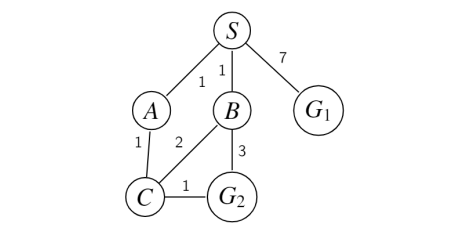
\includegraphics{UCS_question_graph.png}
\\ S is a start state and G1 and G2 are end states. Assume that nodes are searched in alphabetical order. Conduct a BFS and UCS on the graph.
\\ What path does BFS return and what is its cost? What path does UCS return and what is its cost? Produce the overall
results of both search methods as a rigorous proof.
\newpage
% \subsection*{9.3 Answer}
% \addcontentsline{toc}{subsection}{Q9.3 Answer}
% BFS returns the path from S to G1 with a cost of 7. It will push all the neighboring nodes from S, but terminate upon finding that G1 is a goal state and is a neighbor of S.
% \\ UCS returns the path from S to A to C to G2 with a cost of 3. It will first check from S to A and B, being that their cost is 1. Then, it will add the path from S to A to C, because its cost is 2. It will add the paths from S to B to G2 and S to B to C, but those have costs higher than the path from S to A to C. Resuming from S to A to C, it will add the path S to A to C to G2, which will have the lowest cost of any other paths, and then will return that path with cost of 3. 
% \newpage
\subsection*{9.4}
\addcontentsline{toc}{subsection}{Q9.4}
Run $A^*$ search on the following graph, starting at node S and ending at any of the 3 possible goal G nodes. The subscripts on each node are their heuristic values, and you may assume that it is an admissible, consistent heuristic. Show the final search tree and show or explain the state of the priority queue at each step, keeping a closed list of visited nodes.
\begin{center}
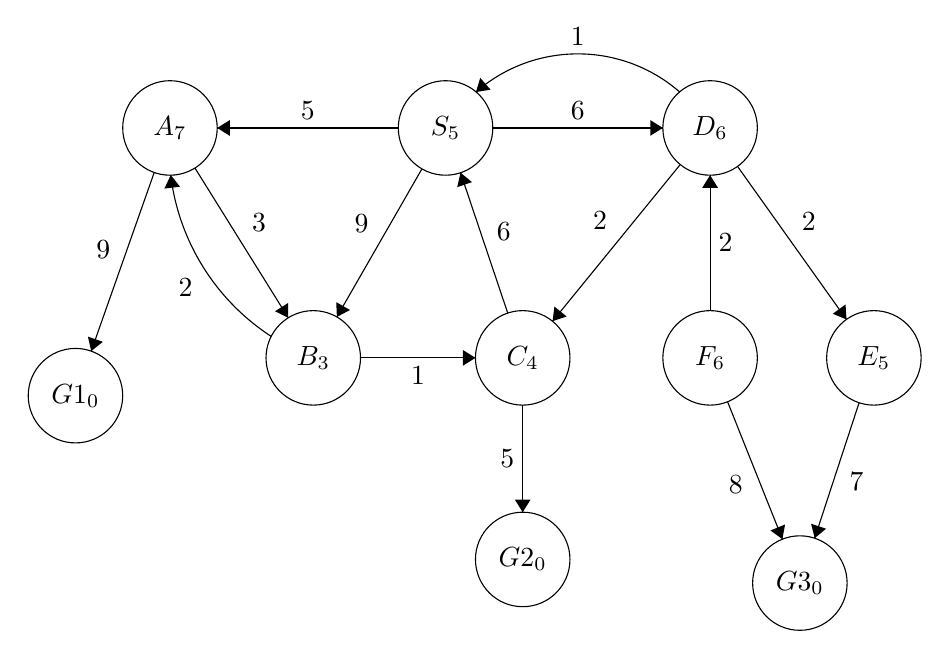
\begin{tikzpicture}[scale=0.2]
\tikzstyle{every node}+=[inner sep=0pt]
\draw [black] (13.2,-8.6) circle (3);
\draw (13.2,-8.6) node {$A_7$};
\draw [black] (22.3,-23.2) circle (3);
\draw (22.3,-23.2) node {$B_3$};
\draw [black] (35.6,-23.2) circle (3);
\draw (35.6,-23.2) node {$C_4$};
\draw [black] (47.5,-8.6) circle (3);
\draw (47.5,-8.6) node {$D_6$};
\draw [black] (57.9,-23.2) circle (3);
\draw (57.9,-23.2) node {$E_5$};
\draw [black] (47.5,-23.2) circle (3);
\draw (47.5,-23.2) node {$F_6$};
\draw [black] (30.7,-8.6) circle (3);
\draw (30.7,-8.6) node {$S_5$};
\draw [black] (7.2,-25.6) circle (3);
\draw (7.2,-25.6) node {$G1_0$};
\draw [black] (35.6,-36) circle (3);
\draw (35.6,-36) node {$G2_0$};
\draw [black] (53.2,-37.5) circle (3);
\draw (53.2,-37.5) node {$G3_0$};
\draw [black] (14.79,-11.15) -- (20.71,-20.65);
\fill [black] (20.71,-20.65) -- (20.71,-19.71) -- (19.87,-20.24);
\draw (18.38,-14.61) node [right] {$3$};
\draw [black] (25.3,-23.2) -- (32.6,-23.2);
\fill [black] (32.6,-23.2) -- (31.8,-22.7) -- (31.8,-23.7);
\draw (28.95,-23.7) node [below] {$1$};
\draw [black] (45.6,-10.93) -- (37.5,-20.87);
\fill [black] (37.5,-20.87) -- (38.39,-20.57) -- (37.61,-19.94);
\draw (40.99,-14.47) node [left] {$2$};
\draw [black] (49.24,-11.04) -- (56.16,-20.76);
\fill [black] (56.16,-20.76) -- (56.1,-19.81) -- (55.29,-20.4);
\draw (53.29,-14.53) node [right] {$2$};
\draw [black] (47.5,-20.2) -- (47.5,-11.6);
\fill [black] (47.5,-11.6) -- (47,-12.4) -- (48,-12.4);
\draw (48,-15.9) node [right] {$2$};
\draw [black] (27.7,-8.6) -- (16.2,-8.6);
\fill [black] (16.2,-8.6) -- (17,-9.1) -- (17,-8.1);
\draw (21.95,-8.1) node [above] {$5$};
\draw [black] (29.2,-11.2) -- (23.8,-20.6);
\fill [black] (23.8,-20.6) -- (24.63,-20.16) -- (23.76,-19.66);
\draw (25.84,-14.67) node [left] {$9$};
\draw [black] (34.65,-20.36) -- (31.65,-11.44);
\fill [black] (31.65,-11.44) -- (31.44,-12.36) -- (32.38,-12.04);
\draw (33.92,-15.19) node [right] {$6$};
\draw [black] (33.7,-8.6) -- (44.5,-8.6);
\fill [black] (44.5,-8.6) -- (43.7,-8.1) -- (43.7,-9.1);
\draw (39.1,-8.1) node [above] {$6$};
\draw [black] (32.63,-6.318) arc (131.05551:48.94449:9.851);
\fill [black] (32.63,-6.32) -- (33.56,-6.17) -- (32.9,-5.42);
\draw (39.1,-3.4) node [above] {$1$};
\draw [black] (56.96,-26.05) -- (54.14,-34.65);
\fill [black] (54.14,-34.65) -- (54.86,-34.05) -- (53.91,-33.73);
\draw (56.32,-31.04) node [right] {$7$};
\draw [black] (48.61,-25.99) -- (52.09,-34.71);
\fill [black] (52.09,-34.71) -- (52.26,-33.78) -- (51.33,-34.16);
\draw (49.6,-31.23) node [left] {$8$};
\draw [black] (35.6,-26.2) -- (35.6,-33);
\fill [black] (35.6,-33) -- (36.1,-32.2) -- (35.1,-32.2);
\draw (35.1,-29.6) node [left] {$5$};
\draw [black] (12.2,-11.43) -- (8.2,-22.77);
\fill [black] (8.2,-22.77) -- (8.94,-22.18) -- (7.99,-21.85);
\draw (9.44,-16.34) node [left] {$9$};
\draw [black] (19.633,-21.839) arc (-123.0476:-173.08284:14.273);
\fill [black] (13.25,-11.59) -- (12.85,-12.45) -- (13.84,-12.33);
\draw (14.67,-18.72) node [left] {$2$};
\end{tikzpicture}
\end{center}
\newpage
% \subsection*{9.4 Answer}
% \addcontentsline{toc}{subsection}{Q9.4 Answer}
% At the start of the algorithm, S is pushed onto the queue with an $A^*$ score of 5. Its outgoing edges are to $A_7$, $B_3$, and $D_6$. However, since $5+7=9+3=6+6=12$, the algorithm considers all paths equal and all three nodes are pushed onto the queue with an $A^*$ score of 12.
% \\ Starting with node A, its outgoing neighbors are B and G1, with $A^*$ scores of 11 and 14, respectively. Both are added to the queue, and since (B, 11) has a higher priority than (B, 12), it is visited first.
% \\ B's outgoing neighbors are A, which has already been visited in a shorter path, and C, which is pushed onto the queue with an $A^*$ score of 13.
% \\ The next highest priority is B again with a score of 12, but this is longer than the (B, 11) path that was already visited, so it goes no further.
% \\ Next priority is (D, 12), whose outgoing neighbors are S (also previously visited with a shorter path), C with a score of 12, and E with a score of 13.
% \\ Next priority is (C, 12), whose outgonig neighbors are S and G2 with a score of 13.
% \\ Next priority is (C, 13), which has already been visited by a shorter path.
% \\ Next priority is (E, 13), whose only outgoing edge is to G3 with a score of 15.
% \\ Now, only paths to the goal are on the priority queue, and so the algorithm returns the path from S to D to C to G2 as the shortest path with a total score of 13.
% \\ Below is the full priority queue and search tree with $A^*$ scores filled in at each node.
% \\ \begin{tabular}{|c|c|c|}
% \hline
%    Pop & Put & Priority Queue \\
% \hline
%   $\empty$ & (S, 5) & (S, 5) \\
% \hline
%   (S, 5) & (A, 12) (B, 12) (D, 12) & (A, 12) (B, 12) (D, 12) \\
% \hline
%   (A, 12) & (B, 11) (G1$_0$, 14) & (B, 11) (B, 12) (D, 12) (G1$_0$, 14) \\
% \hline
%   (B, 11) & (C, 13) & (B, 11) (B, 12) (D, 12) (C, 13) (G1$_0$, 14) \\
% \hline
%   (B, 12) & & (D, 12) (C, 13) (G1$_0$, 14) \\
% \hline
%   (D, 12) & (C, 12) (E, 13) & (C,12) (C, 13) (E, 13) (G1$_0$, 14) \\
% \hline
%   (C, 12) & (G2$_0$, 13) & (C, 13) (E, 13) (G2$_0$, 13) (G1$_0$, 14) \\
% \hline
%   (C, 13) &  & (E, 13) (G2$_0$, 13) (G1$_0$, 14) \\
% \hline
%   (E, 13) & (G3, 15) & (G2$_0$, 13) (G1$_0$, 14) (G3, 15) \\
% \hline
% \end{tabular}
% \begin{center}
% \begin{tikzpicture}[scale=0.2]
% \tikzstyle{every node}+=[inner sep=0pt]
% \draw [black] (35.1,-6.1) circle (3);
% \draw (35.1,-6.1) node {$S_5$};
% \draw [black] (21.5,-17.7) circle (3);
% \draw (21.5,-17.7) node {$A_7:12$};
% \draw [black] (35.1,-17.7) circle (3);
% \draw (35.1,-17.7) node {$B_3:12$};
% \draw [black] (50.2,-17.7) circle (3);
% \draw (50.2,-17.7) node {$D_6:12$};
% \draw [black] (16.4,-27.7) circle (3);
% \draw (16.4,-27.7) node {$B_3:11$};
% \draw [black] (27.2,-27.7) circle (3);
% \draw (27.2,-27.7) node {$G1_0:14$};
% \draw [black] (16.4,-39.3) circle (3);
% \draw (16.4,-39.3) node {$C_4:13$};
% \draw [black] (44,-27.7) circle (3);
% \draw (44,-27.7) node {$C_4:12$};
% \draw [black] (57,-27.7) circle (3);
% \draw (57,-27.7) node {$E_5:13$};
% \draw [black] (57,-39.3) circle (3);
% \draw (57,-39.3) node {$G3_0:15$};
% \draw [black] (44,-38.6) circle (3);
% \draw (44,-38.6) node {$G2_0:13$};
% \draw [black] (32.82,-8.05) -- (23.78,-15.75);
% \fill [black] (23.78,-15.75) -- (24.72,-15.61) -- (24.07,-14.85);
% \draw (27.29,-11.41) node [above] {$5$};
% \draw [black] (35.1,-9.1) -- (35.1,-14.7);
% \fill [black] (35.1,-14.7) -- (35.6,-13.9) -- (34.6,-13.9);
% \draw (34.6,-11.9) node [left] {$9$};
% \draw [black] (37.48,-7.93) -- (47.82,-15.87);
% \fill [black] (47.82,-15.87) -- (47.49,-14.99) -- (46.88,-15.78);
% \draw (43.66,-11.4) node [above] {$6$};
% \draw [black] (20.14,-20.37) -- (17.76,-25.03);
% \fill [black] (17.76,-25.03) -- (18.57,-24.54) -- (17.68,-24.09);
% \draw (18.26,-21.57) node [left] {$3$};
% \draw [black] (22.99,-20.31) -- (25.71,-25.09);
% \fill [black] (25.71,-25.09) -- (25.75,-24.15) -- (24.88,-24.65);
% \draw (25.01,-21.48) node [right] {$9$};
% \draw [black] (16.4,-30.7) -- (16.4,-36.3);
% \fill [black] (16.4,-36.3) -- (16.9,-35.5) -- (15.9,-35.5);
% \draw (15.9,-33.5) node [left] {$1$};
% \draw [black] (44,-30.7) -- (44,-35.6);
% \fill [black] (44,-35.6) -- (44.5,-34.8) -- (43.5,-34.8);
% \draw (43.5,-33.15) node [left] {$5$};
% \draw [black] (57,-30.7) -- (57,-36.3);
% \fill [black] (57,-36.3) -- (57.5,-35.5) -- (56.5,-35.5);
% \draw (56.5,-33.5) node [left] {$7$};
% \draw [black] (51.89,-20.18) -- (55.31,-25.22);
% \fill [black] (55.31,-25.22) -- (55.28,-24.28) -- (54.45,-24.84);
% \draw (54.2,-21.35) node [right] {$2$};
% \draw [black] (48.62,-20.25) -- (45.58,-25.15);
% \fill [black] (45.58,-25.15) -- (46.43,-24.73) -- (45.58,-24.21);
% \draw (46.47,-21.41) node [left] {$2$};
% \end{tikzpicture}
% \end{center}
% \newpage
% \subsection*{Additional Resources for Graphs and Trees}
% \addcontentsline{toc}{subsection}{Additional Resources}
% \begin{enumerate}
%     \item \href{https://www.youtube.com/watch?v=zaBhtODEL0w}{DFS and BFS}
%     \item \href{https://www.youtube.com/watch?v=DgXR2OWQnLc&list=PLDV1Zeh2NRsDGO4--qE8yH72HFL1Km93P}{Graph Theory Playlist}
%     \item \href{https://www.youtube.com/watch?v=dRMvK76xQJI}{Uniform Cost Search}
%     \item \href{https://www.youtube.com/watch?v=6TsL96NAZCo}{A* Search}
% \end{enumerate}
% \newpage
\section*{Chapter 5: Regular Expressions}
\addcontentsline{toc}{section}{Chapter 5: Regular Expressions}

\subsection*{Q5.1}
\addcontentsline{toc}{subsection}{Q5.1}
Assume the alphabet $\sum=\{0,1\}$. If the English description is given, provide the regular expression. If the regular expression is given, give a short, English description of the accepted set of strings.
\begin{enumerate}[label=\alph*.]
    \item The set of strings that contain at least one 0 and at least one 1.
    \item $(1+\lambda)(00^*1)^*0^*$
    \item The set of strings such that all pairs of adjacent 0's appear before any pairs of adjacent 1's.
\end{enumerate}
\newpage
% \subsection*{Q5.1 Answer}
% \addcontentsline{toc}{subsection}{Q5.1 Answer}
% \begin{enumerate}[label=\alph*.]
%     \item This can be thought of as either a 0 appearing before the 1, or the 1 appearing before the 0. Since these are the only mandated characters, the rest of the string can be any combination of 0's and 1's that come before, in-between, or after the 0 and 1. In other words, there are two possible string formats: $(0+1)^*0(0+1)^*1(0+1)^*$ or $(0+1)^*1(0+1)^*0(0+1)^*$
%     \\ Together, the full regex is $((0+1)^*0(0+1)^*1(0+1)^*)+((0+1)^*1(0+1)^*0(0+1)^*)$
%     \item The language starts with either a 1 or an empty string. From there, it is followed by a 0, some number of zero's, and then a 1. Just looking at these parts, the string can start as either:
%     \\ 1 0 0... 1 
%     \\ 0 0... 1
%     \\ Even if the 0... is omitted, the string can only start with 0 1. 1 1 is not allowed.
%     \\ Looking further, we can observe that within the $(00^*1)$ part, removing the optional 0's, $(01)$ the structure mandates that 0 must come before 1. So if this block repeats, the structure will looks like this: 0 1 0 1 with more 0's padding the in-between. And since only more 0's are added onto the end, we can conclude that this will be the set of all strings without consecutive 1's.
%     \item This can be divided into two parts: The first part of the string that does not allow 11's, but does allow 00's, and the second part of the string that does not allow 00's, but does allow 11's.
%     \\ For a binary string where 11 cannot occur, this could be any combination of 0's or 10's, either ending in a 1 or not: $(0+10)^*(1+\lambda)$
%     \\ The formula is much the same for a binary string where 00 cannot occur: $(1+01)^*(0+\lambda)$
%     \\ Concatenating the two together gives us the final string: $(0+10)^*(1+\lambda)(1+01)^*(0+\lambda)$
% \end{enumerate}
% \newpage
\subsection*{Q5.2}
\addcontentsline{toc}{subsection}{Q5.2}
Is the Kleene star operation distributive over the + operation? In other words, is $(S+T)^*=S^*+T^*$ true for any languages S and T? Why or why not?
\\ If your answer is no, is this always true, or can you think of specific values for S and T that would make it true?
\newpage
% \subsection*{Q5.2 Answer}
% \addcontentsline{toc}{subsection}{Q5.2 Answer}
% No, they are not. $(S+T)^*$ indicates choosing between S and T, and then repeatedly concatenating this any number of times. Therefore, it produces combination strings that can switch between S and T. However, $S^*+T^*$ only chooses between S and T after the repeated concatenations, and so it cannot produce strings with combinations of S and T---it can only produce strings that are either repeated concatenations of S or repeated concatenations of T. 
% \\ The above is generally true, but when either S or T (or both) are the empty language, or when S and T are the same language, $(S+T)^*=S^*+T^*$.
% \newpage
% \subsection*{Additional Resources for Regular Expressions}
% \addcontentsline{toc}{subsection}{Additional Resources}
% \begin{enumerate}
%     \item \href{https://www.youtube.com/playlist?list=PLBlnK6fEyqRgp46KUv4ZY69yXmpwKOIev}{Formal Language Theory Playlist}
% \end{enumerate}
% \newpage

\section*{Chapter 14: Finite Automata}
\addcontentsline{toc}{section}{Chapter 14: Finite Automata}

\subsection*{Q14.1}
\addcontentsline{toc}{subsection}{Q14.1}
Assume $\sum=\{0,1\}$. Draw a DFA for the language that accepts all binary strings with either an even number of 0's or contains exactly two 1's.
\newpage
% \subsection*{Q14.1 Answer}
% \addcontentsline{toc}{subsection}{Q14.1 Answer}
% Let us first consider what states this machine will need. The machine considers strings based on two different criteria, although a string only needs one to be accepted. The first condition is that there is an even number of 0's. There are only two states for this, an even number of 0's or an odd number of 0's. Reading in 0's would switch between the two states like so:
% \begin{center}
% \begin{tikzpicture}[scale=0.2]
% \tikzstyle{every node}+=[inner sep=0pt]
% \draw [black] (26,-20.8) circle (3);
% \draw (26,-20.8) node {even};
% \draw [black] (26,-20.8) circle (2.4);
% \draw [black] (43.2,-20.8) circle (3);
% \draw (43.2,-20.8) node {odd};
% \draw [black] (41.348,-23.145) arc (-46.98484:-133.01516:9.892);
% \fill [black] (41.35,-23.15) -- (40.42,-23.33) -- (41.1,-24.06);
% \draw (34.6,-26.3) node [below] {$0$};
% \draw [black] (40.2,-20.8) -- (29,-20.8);
% \fill [black] (29,-20.8) -- (29.8,-21.3) -- (29.8,-20.3);
% \draw (34.6,-20.3) node [above] {$0$};
% \draw [black] (14.4,-20.8) -- (23,-20.8);
% \fill [black] (23,-20.8) -- (22.2,-20.3) -- (22.2,-21.3);
% \end{tikzpicture}
% \end{center}
% Now let us consider the other criteria, which is "exactly two 1's". This has four states: zero 1's, exactly one 1, exactly two 1's, and more than two 1's, since beyond two 1's, that criteria will always fail. Reading in any 1 will move between these states, ending with the "more than two 1's" state in a dead end.
% \begin{center}
% \begin{tikzpicture}[scale=0.2]
% \tikzstyle{every node}+=[inner sep=0pt]
% \draw [black] (28.9,-20.3) circle (3);
% \draw (28.9,-20.3) node {$1$};
% \draw [black] (40.3,-20.3) circle (3);
% \draw (40.3,-20.3) node {$2$};
% \draw [black] (40.3,-20.3) circle (2.4);
% \draw [black] (52.2,-20.3) circle (3);
% \draw (52.2,-20.3) node {$>2$};
% \draw [black] (17.9,-20.3) circle (3);
% \draw (17.9,-20.3) node {$0$};
% \draw [black] (31.9,-20.3) -- (37.3,-20.3);
% \fill [black] (37.3,-20.3) -- (36.5,-19.8) -- (36.5,-20.8);
% \draw (34.6,-20.8) node [below] {$1$};
% \draw [black] (43.3,-20.3) -- (49.2,-20.3);
% \fill [black] (49.2,-20.3) -- (48.4,-19.8) -- (48.4,-20.8);
% \draw (46.25,-20.8) node [below] {$1$};
% \draw [black] (20.9,-20.3) -- (25.9,-20.3);
% \fill [black] (25.9,-20.3) -- (25.1,-19.8) -- (25.1,-20.8);
% \draw (23.4,-20.8) node [below] {$1$};
% \draw [black] (8.4,-20.3) -- (14.9,-20.3);
% \fill [black] (14.9,-20.3) -- (14.1,-19.8) -- (14.1,-20.8);
% \draw [black] (50.877,-17.62) arc (234:-54:2.25);
% \draw (52.2,-13.05) node [above] {$1$};
% \fill [black] (53.52,-17.62) -- (54.4,-17.27) -- (53.59,-16.68);
% \end{tikzpicture}
% \end{center}
% Since one criteria only cares about 0's being read in, and the other only cares about 1's being read in, we can combine the two into one machine with 8 states, each representing a state from the even/odd criteria \textit{and} a state from the "how many 1's" criteria.
% \begin{center}
%     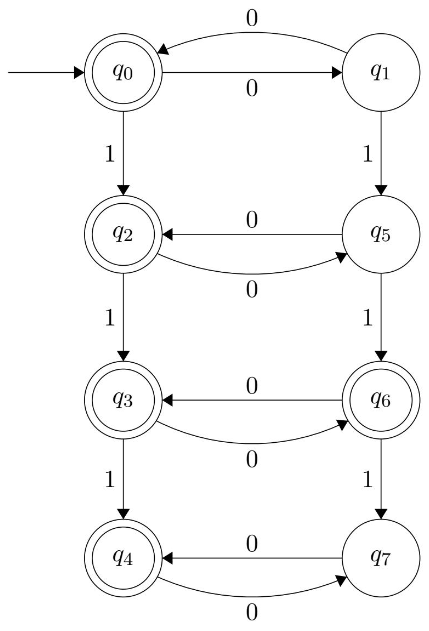
\includegraphics[width=6cm]{Screenshot 2023-11-21 143618.png}
% \end{center}
% \newpage

\subsection*{Q14.2}
\addcontentsline{toc}{subsection}{Q14.2}
Construct a DFA that accepts a language consisting of all strings over the alphabet \(\Sigma=\{a, b\}\) that either end with the letter 'a' or contain an even number of 'b's.
\newpage
% \subsection*{Q14.2 Answer}
% \addcontentsline{toc}{subsection}{Q14.2 Answer}
% The given diagram represents a DFA comprising five states, \( s_0 \) to \( s_4 \), with \( s_0 \) as the start state and \( s_2 \), \( s_4 \) as accept states. The transitions are defined by the input symbols 'a' and 'b':
% \begin{itemize}
%     \item From \( s_0 \), there is a transition to \( s_1 \) on input 'a' and a loop on 'b'.
%     \item State \( s_1 \) transitions to \( s_2 \) on 'a' and to \( s_3 \) on 'b'.
%     \item State \( s_2 \) has a loop on 'a'.
%     \item State \( s_3 \) transitions to \( s_1 \) on 'a' and to \( s_4 \) on 'b'.
%     \item State \( s_4 \) has a loop on 'b'.
% \end{itemize}
% This DFA accepts strings that end with 'a' leading to \( s_2 \) or strings with an even number of 'b's leading to \( s_4 \).
% \begin{center}
%     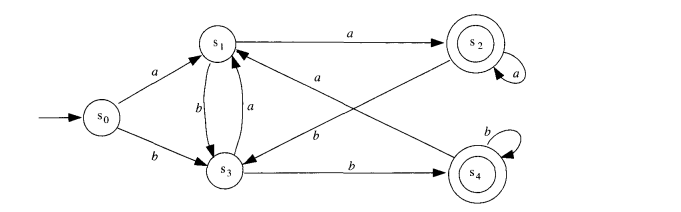
\includegraphics[width=15cm]{1.png}
% \end{center}
% \newpage

\subsection*{Q14.3}
\addcontentsline{toc}{subsection}{Q14.3}
Use the DFA minimization algorithm on the following DFA:
\begin{center}
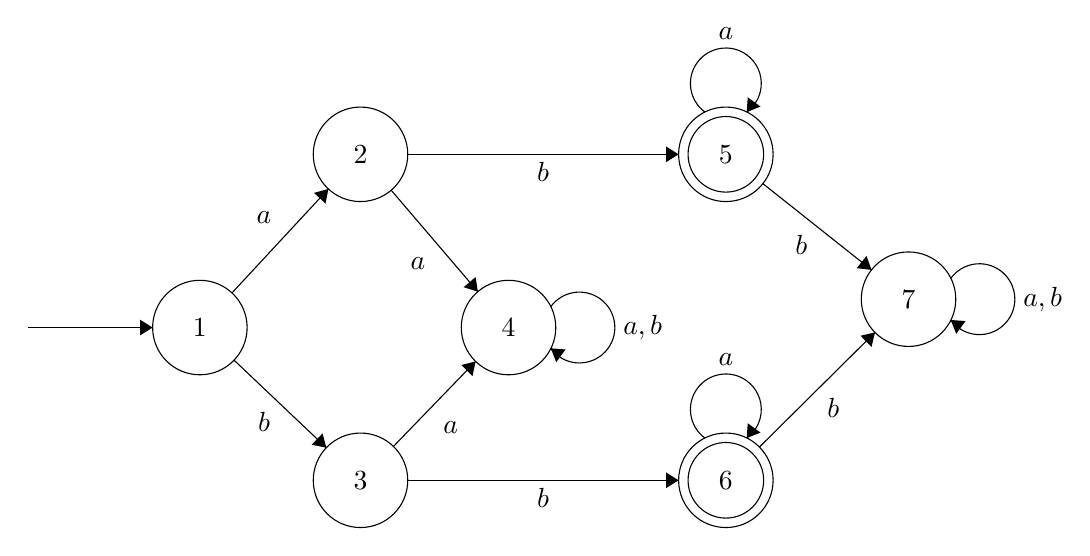
\begin{tikzpicture}[scale=0.2]
\tikzstyle{every node}+=[inner sep=0pt]
\draw [black] (12.7,-30) circle (3);
\draw (12.7,-30) node {$1$};
\draw [black] (22.9,-19) circle (3);
\draw (22.9,-19) node {$2$};
\draw [black] (22.9,-39.7) circle (3);
\draw (22.9,-39.7) node {$3$};
\draw [black] (32.3,-30) circle (3);
\draw (32.3,-30) node {$4$};
\draw [black] (46.1,-19) circle (3);
\draw (46.1,-19) node {$5$};
\draw [black] (46.1,-19) circle (2.4);
\draw [black] (46.1,-39.7) circle (3);
\draw (46.1,-39.7) node {$6$};
\draw [black] (46.1,-39.7) circle (2.4);
\draw [black] (57.7,-28.2) circle (3);
\draw (57.7,-28.2) node {$7$};
\draw [black] (1.8,-30) -- (9.7,-30);
\fill [black] (9.7,-30) -- (8.9,-29.5) -- (8.9,-30.5);
\draw [black] (14.74,-27.8) -- (20.86,-21.2);
\fill [black] (20.86,-21.2) -- (19.95,-21.45) -- (20.68,-22.13);
\draw (17.27,-23.04) node [left] {$a$};
\draw [black] (14.87,-32.07) -- (20.73,-37.63);
\fill [black] (20.73,-37.63) -- (20.49,-36.72) -- (19.8,-37.44);
\draw (16.78,-35.33) node [below] {$b$};
\draw [black] (24.99,-37.55) -- (30.21,-32.15);
\fill [black] (30.21,-32.15) -- (29.3,-32.38) -- (30.01,-33.08);
\draw (28.13,-36.32) node [right] {$a$};
\draw [black] (25.9,-39.7) -- (43.1,-39.7);
\fill [black] (43.1,-39.7) -- (42.3,-39.2) -- (42.3,-40.2);
\draw (34.5,-40.2) node [below] {$b$};
\draw [black] (44.777,-37.02) arc (234:-54:2.25);
\draw (46.1,-32.45) node [above] {$a$};
\fill [black] (47.42,-37.02) -- (48.3,-36.67) -- (47.49,-36.08);
\draw [black] (48.23,-37.59) -- (55.57,-30.31);
\fill [black] (55.57,-30.31) -- (54.65,-30.52) -- (55.35,-31.23);
\draw (52.92,-34.43) node [below] {$b$};
\draw [black] (60.38,-26.877) arc (144:-144:2.25);
\draw (64.95,-28.2) node [right] {$a,b$};
\fill [black] (60.38,-29.52) -- (60.73,-30.4) -- (61.32,-29.59);
\draw [black] (48.45,-20.86) -- (55.35,-26.34);
\fill [black] (55.35,-26.34) -- (55.03,-25.45) -- (54.41,-26.23);
\draw (50.89,-24.1) node [below] {$b$};
\draw [black] (44.777,-16.32) arc (234:-54:2.25);
\draw (46.1,-11.75) node [above] {$a$};
\fill [black] (47.42,-16.32) -- (48.3,-15.97) -- (47.49,-15.38);
\draw [black] (25.9,-19) -- (43.1,-19);
\fill [black] (43.1,-19) -- (42.3,-18.5) -- (42.3,-19.5);
\draw (34.5,-19.5) node [below] {$b$};
\draw [black] (34.98,-28.677) arc (144:-144:2.25);
\draw (39.55,-30) node [right] {$a,b$};
\fill [black] (34.98,-31.32) -- (35.33,-32.2) -- (35.92,-31.39);
\draw [black] (24.85,-21.28) -- (30.35,-27.72);
\fill [black] (30.35,-27.72) -- (30.21,-26.79) -- (29.45,-27.44);
\draw (27.05,-25.94) node [left] {$a$};
\end{tikzpicture}
\end{center}
\newpage
% \subsection*{Q14.3 Answer}
% \addcontentsline{toc}{subsection}{Q14.3 Answer}
% The DFA minimization algorithm begins by separating the nodes into accept states and non-accept states. Each of these groups is called a "class", and each iteration of this algorithm is called a relation. The point of the algorithm is to divide each class up into smaller and smaller groups of nodes until they cannot be divided anymore, meaning we have reached the minimal DFA.
% \\ Relation 0: Class A = $\{1,2,3,4,7\}$ Class B = $\{5,6\}$
% \\ Below, we have a table showing each node in each class and which class its edges point towards. Nodes 2 and 3 have a different behavior than the other nodes in A---when reading in a 'b', they lead to class B, not class A. So we will separate out those nodes into their own class in the next iteration.
% \\ \begin{tabular}{c|c|c}
%  Node & Class ($a$ input) & Class ($b$ input) \\
% \hline
%  1 & A & A \\
%  2 & A & B \\
%  3 & A & B \\
%  4 & A & A \\
%  7 & A & A \\
% \hline
%  5 & B & A \\
%  6 & B & A \\
% \end{tabular}
% \\ Relation 1: Class A = $\{1,4,7\}$ Class B = $\{5,6\}$ Class C = $\{2,3\}$
% \\ In the below table, we relabel the edges to reflect the new classes, and once again observe that node 1's behavior is unlike the others in Class A. Therefore, again, we put it in its own separate class.
% \\ \begin{tabular}{c|c|c}
%  Node & Class ($a$ input) & Class ($b$ input) \\
% \hline
%  1 & C & C \\
%  4 & A & A \\
%  7 & A & A \\
% \hline
%  2 & A & B \\
%  3 & A & B \\
% \hline
%  5 & B & A \\
%  6 & B & A \\
% \end{tabular}
% \\ Relation 2: Class A = $\{4,7\}$ Class B = $\{5,6\}$ Class C = $\{2,3\}$ Class D = $\{1\}$
% \\ In the below table, we relabel the edges to reflect the new classes, and once again observe that node 1's behavior is unlike the others in Class A. Therefore, again, we put it in its own separate class.
% \\ \begin{tabular}{c|c|c}
%  Node & Class ($a$ input) & Class ($b$ input) \\
% \hline
%  1 & C & C \\
% \hline
%  4 & A & A \\
%  7 & A & A \\
% \hline
%  2 & A & B \\
%  3 & A & B \\
% \hline
%  5 & B & A \\
%  6 & B & A \\
% \end{tabular}
% \\ We have now reached the end of the minimization algorithm, since all behaviors in each class are the same, meaning all the nodes in each class can be condensed into a single node with one uniform output and input that is representative of all the nodes within. The minimal DFA is shown below.
% \begin{center}
% \begin{tikzpicture}[scale=0.2]
% \tikzstyle{every node}+=[inner sep=0pt]
% \draw [black] (12.7,-30) circle (3);
% \draw (12.7,-30) node {$D$};
% \draw [black] (26.3,-30) circle (3);
% \draw (26.3,-30) node {$C$};
% \draw [black] (34.1,-13.2) circle (3);
% \draw (34.1,-13.2) node {$A$};
% \draw [black] (42.8,-30) circle (3);
% \draw (42.8,-30) node {$B$};
% \draw [black] (42.8,-30) circle (2.4);
% \draw [black] (1.8,-30) -- (9.7,-30);
% \fill [black] (9.7,-30) -- (8.9,-29.5) -- (8.9,-30.5);
% \draw [black] (15.7,-30) -- (23.3,-30);
% \fill [black] (23.3,-30) -- (22.5,-29.5) -- (22.5,-30.5);
% \draw (19.5,-29.5) node [above] {$a,b$};
% \draw [black] (29.3,-30) -- (39.8,-30);
% \fill [black] (39.8,-30) -- (39,-29.5) -- (39,-30.5);
% \draw (34.55,-30.5) node [below] {$b$};
% \draw [black] (27.56,-27.28) -- (32.84,-15.92);
% \fill [black] (32.84,-15.92) -- (32.05,-16.44) -- (32.95,-16.86);
% \draw (30.92,-22.64) node [right] {$a$};
% \draw [black] (32.777,-10.52) arc (234:-54:2.25);
% \draw (34.1,-5.95) node [above] {$a,b$};
% \fill [black] (35.42,-10.52) -- (36.3,-10.17) -- (35.49,-9.58);
% \draw [black] (41.42,-27.34) -- (35.48,-15.86);
% \fill [black] (35.48,-15.86) -- (35.4,-16.8) -- (36.29,-16.34);
% \draw (39.14,-20.46) node [right] {$b$};
% \draw [black] (45.48,-28.677) arc (144:-144:2.25);
% \draw (50.05,-30) node [right] {$a$};
% \fill [black] (45.48,-31.32) -- (45.83,-32.2) -- (46.42,-31.39);
% \end{tikzpicture}
% \end{center}
% \newpage

\subsection*{Q14.4}
\addcontentsline{toc}{subsection}{Q14.4}
Convert the following NFA to a DFA:
\begin{center}
    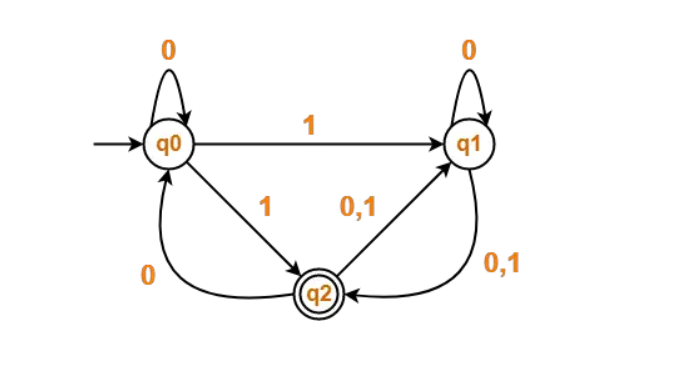
\includegraphics[width=12cm]{13.png}
\end{center}
\newpage
% \subsection*{Q14.4 Answer}
% \addcontentsline{toc}{subsection}{Q14.4 Answer}
% \begin{table}[h]
% \centering
% \begin{tabular}{c|c|c}
% State / Alphabet & 0 & 1 \\ \hline
% $\rightarrow q_0$ & $q_0$ & $q_1, *q_2$ \\
% $q_1$ & $q_1, *q_2$ & $*q_2$ \\
% $*q_2$ & $q_0, q_1$ & $q_1$ \\
% \end{tabular}
% \caption{Transition table for the given NFA}
% \end{table}
% \textbf{Step 1}
% \begin{enumerate}
% \item Let $Q'$ be a new set of states of the Deterministic Finite Automata (DFA).
% \item Let $T'$ be a new transition table of the DFA.
% \end{enumerate}
% \textbf{Step 2}
% \\ Add transitions of start state $q_0$ to the transition table $T'$.
% \begin{table}[h]
% \centering
% \begin{tabular}{c|c|c}
% State / Alphabet & 0 & 1 \\ \hline
% $\rightarrow q_0$ & $q_0$ & $\{q_1, q_2\}$ \\
% \end{tabular}
% \caption{Partial transition table for DFA}
% \end{table}
% \\ \textbf{Step 3}
% \begin{enumerate}
% \item New state present in state $Q'$ is $\{q_1, q_2\}$.
% \item Add transitions for set of states $\{q_1, q_2\}$ to the transition table $T'$.
% \end{enumerate}
% \begin{table}[h]
% \centering
% \begin{tabular}{c|c|c}
% State / Alphabet & 0 & 1 \\ \hline
% $\rightarrow q_0$ & $q_0$ & $\{q_1, q_2\}$ \\
% $\{q_1, q_2\}$ & $\{q_0, q_1, q_2\}$ & $\{q_1, q_2\}$ \\
% \end{tabular}
% \caption{Extended transition table for DFA}
% \end{table}
% \textbf{Step 4}
% \begin{enumerate}
% \item New state present in state $Q'$ is $\{q_0, q_1, q_2\}$.
% \item Add transitions for set of states $\{q_0, q_1, q_2\}$ to the transition table $T'$.
% \end{enumerate}
% \begin{table}[h]
% \centering
% \begin{tabular}{c|c|c}
% State / Alphabet & 0 & 1 \\ \hline
% $\rightarrow q_0$ & $q_0$ & $\{q_1, q_2\}$ \\
% $\{q_1, q_2\}$ & $\{q_0, q_1, q_2\}$ & $\{q_1, q_2\}$ \\
% $\{q_0, q_1, q_2\}$ & $\{q_0, q_1, q_2\}$ & $\{q_1, q_2\}$ \\
% \end{tabular}
% \caption{Extended transition table for DFA}
% \end{table}
% \textbf{Step 5}
% \begin{enumerate}
% \item Since no new states are left to be added in the transition table $T'$, we stop.
% \item States containing $q_2$ as its component are treated as final states of the DFA.
% \end{enumerate}
% Finally, the transition table for Deterministic Finite Automata (DFA) is:
% \begin{table}[h]
% \centering
% \begin{tabular}{c|c|c}
% State / Alphabet & 0 & 1 \\ \hline
% $\rightarrow q_0$ & $q_0$ & $*\{q_1, q_2\}$ \\
% $*\{q_1, q_2\}$ & $*\{q_0, q_1, q_2\}$ & $*\{q_1, q_2\}$ \\
% $*\{q_0, q_1, q_2\}$ & $*\{q_0, q_1, q_2\}$ & $*\{q_1, q_2\}$ \\
% \end{tabular}
% \caption{Transition table for the DFA}
% \end{table}
% \begin{center}
%     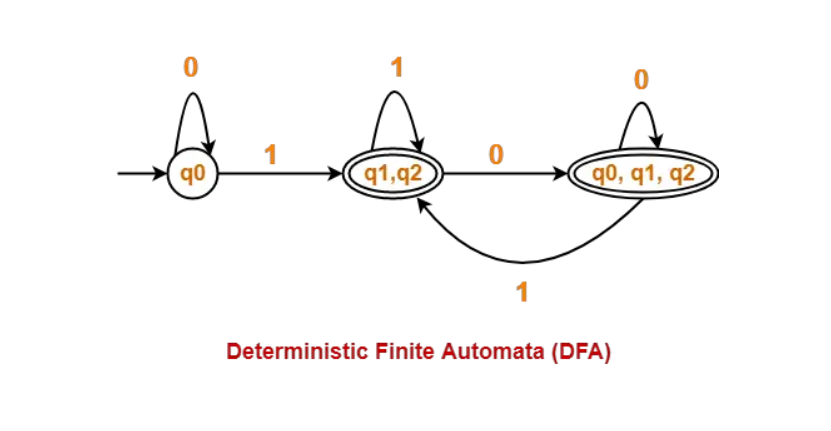
\includegraphics[width=12cm]{14.png}
% \end{center}
% \newpage
\subsection*{Q14.5}
\addcontentsline{toc}{subsection}{Q14.5}
Let $L^R$ be any arbitrary regular language. Let the language $L^R = \{w^R : w \in L\}$ be the reversal of L.
Show that $L^R$ is regular.
\newpage
% \subsection*{Q14.5 Answer}
% \addcontentsline{toc}{subsection}{Q14.5 Answer}
% Since we know that $L$ is regular, we know that there exists some DFA or equivalent $\lambda$-NFA which accepts $L$. Without loss of generality, we can
% assume that there exists only start or end state (If a DFA had multiple accepting states, you could eliminate them down to just one 
% by redirecting all of the arrows going into other accepting states into a single accepting state, and eliminating the redundant accepting
% states). Then we can construct a DFA or equivalent $\lambda$-NFA which accepts $L^R$ by making the start state and accepting state, the accepting state
% a start state, and reversing every state transition (reversing the "arrows"). Then we have a machine that traverses backwards over every
% string in $L$, and have thus constructed a DFA for $L^R$. Since there exists a DFA / $\lambda$-NFA for $L^R$, we know that $L^R$ is regular.
% \newpage
\subsection*{Q14.6}
\addcontentsline{toc}{subsection}{Q14.6}
For $\Sigma=\{a,b,c,d\}$, give a regular expression that captures all strings that use their letters in reverse alphabetical order, but use at most three of the four possible letters.
\\ Note: The strings themselves can be longer than 3 letters long, since letters can repeat.
 Draw an NFA that captures the regular expression from above.
\newpage
% \subsection*{Q14.6 Answer}
% \addcontentsline{toc}{subsection}{Q14.6 Answer}
% The regular expression that captures the above language is:
% \[(d^*c^*b^*)+(d^*b^*a^*)+(d^*c^*a^*)+(c^*b^*a^*)\]
% We will construct this NFA step by step. Initially, consider the NFA for \( a^* \) as follows:
% \begin{center}
%     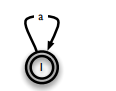
\includegraphics[width=4cm]{10.png}
% \end{center}
% The NFA for \( d^*c^*b^* \) is constructed by chaining the NFAs for \( d^* \), \( c^* \), and \( b^* \) as shown:
% \begin{center}
%     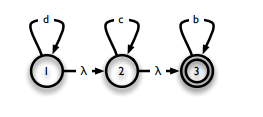
\includegraphics[width=9cm]{11.png}
% \end{center}
% Extra care is taken when connecting the NFAs sequentially; the final states of the first NFA are connected to the start state of the subsequent NFA, and the final states are made non-final to ensure the correctness of the overall NFA. Although it is safe to keep all states final in this specific case, it is generally prudent not to do so in order to avoid errors in the construction of the NFA.
% Now we can combine the components to construct the overall NFA.
% \begin{center}
%     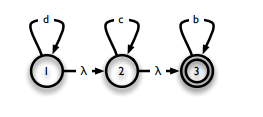
\includegraphics[width=9cm]{11.png}
% \end{center}
% \newpage

% \subsection*{Q14.7}
% \addcontentsline{toc}{subsection}{Q14.7}
% Let \( L_1L_2 \) be the set of strings of 0's and 1's that both start and end with a 0.
% \\ Let \( L_1 \cup L_2 \) be the set of strings of 0's and 1's that start with a 0 or end with a 0 (or both).
% \\ Then the language \( (L_1 \cup L_2)^* \) is the set of strings of 0's and 1's that start with a 0 or end with a 0 (or both) or that contain 00.
% \newpage
% \subsection*{Q14.7 Answer}
% \addcontentsline{toc}{subsection}{Q14.7 Answer}
% \begin{center}
%     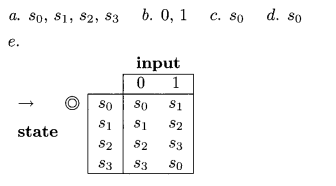
\includegraphics[width=10cm]{2.png}
% \end{center}
% \newpage

% \subsection*{Q14.8}
% \addcontentsline{toc}{subsection}{Q14.8}
% Determining the transition from state \( S_2 \) on inputs \( a \) and \( b \) is straightforward; from the empty set of states, there are no transitions in the NFA. In the DFA, this is represented by a transition from the empty set back to itself.
% \begin{center}
%     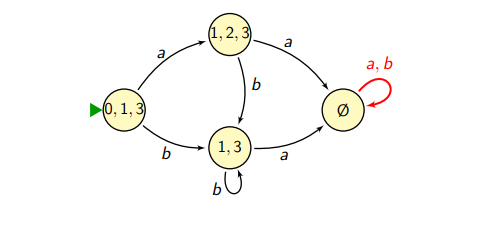
\includegraphics[width=12cm]{6.png}
% \end{center}
% \newpage
% \subsection*{Q14.8 Answer}
% \addcontentsline{toc}{subsection}{Q14.6 Answer}
% \begin{center}
%     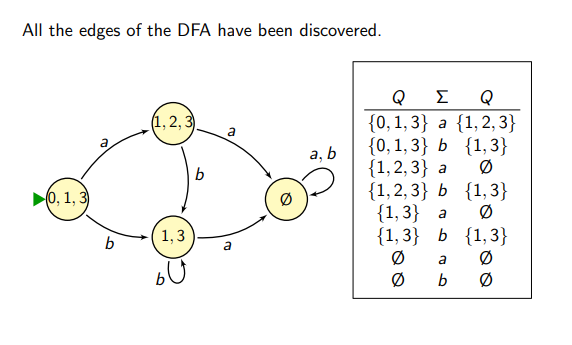
\includegraphics[width=12cm]{7.png}
% \end{center}
% \begin{center}
%     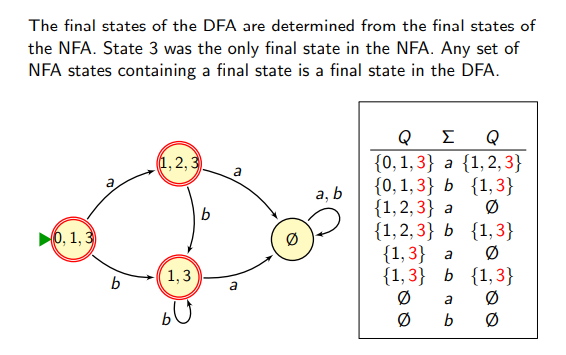
\includegraphics[width=12cm]{8.png}
% \end{center}
% \begin{center}
%    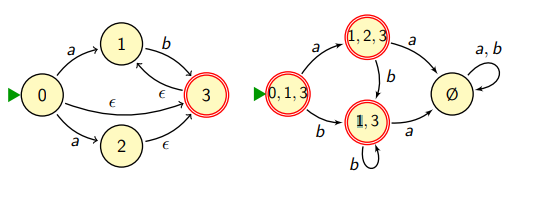
\includegraphics[width=12cm]{9.png}
% \end{center}
% \newpage

\subsection*{Additional Resourches for Finite Automata}
\addcontentsline{toc}{subsection}{Additional Resources}
\begin{enumerate}
    \item \href{https://www.youtube.com/watch?v=gjDPTy6fwbk}{Myhill Nerode}
    \item \href{https://www.youtube.com/watch?v=7W2lSrt8r-0&t=703s}{DFA Minimization}
    \item \href{https://www.youtube.com/watch?v=VbR1mGdP99s}{Regular Expression to Automaton}
    \item \href{https://www.youtube.com/watch?v=yXLZ9JbvEEg}{Lambda/Epsilon NFA to NFA}
\end{enumerate}
\newpage

\section*{Chapter 15: Formal Language Theory}
\addcontentsline{toc}{section}{Chapter 15: Formal Language Theory}

\subsection*{Q15.1}
\addcontentsline{toc}{subsection}{Q15.1}
Let L be a language that is Turing Recognizable by some Turing Machine. Let L' be the language $\Sigma^* - L$,
and let that language also be Turing Recognizable by some other Turing Machine. Prove that L is Turing Decidable.
(Hint: Recall that a single-tape Turing Machine can be used to simulate a multi-tape Turing Machine)
\newpage
% \subsection*{Q15.1 Answer}
% \addcontentsline{toc}{subsection}{Q15.1 Answer}
% We know this to be true by the TR / TD Theorem. But for a rigorous proof, recall that a multi-tape Turing Machine can be simulated by
% a single-tape Turing Machine. Then we will construct a multi-tape Turing Machine which runs the Turing Machines for L and L' in parallel. One of these
% is guaranteed to terminate, since $L + L' = \Sigma^*$. If, on any given string, the Turing Machine that recognizes L terminates, 
% we know that string is in L. If the Turing Machine that recognizes L' terminates, we know that string is not in L. Then here we have
% constructed a Turing Machine that always decides whether or not a string is in L, and so L is Turing Decidable.
% \newpage

\subsection*{Additional Resources for Formal Language Theory}
\addcontentsline{toc}{subsection}{Additional Resources}
\begin{enumerate}
    \item \href{https://www.youtube.com/watch?v=-ZS_zFg4w5k}{Turing Machines Visualized}
    \item \href{https://www.youtube.com/watch?v=sNWC1Zz6qcg}{TR / TD}
    \item \href{https://www.youtube.com/watch?v=VyHbd6sx5Po}{Halting Problem}
    \item \href{https://www.youtube.com/watch?v=SV57Yv8BXBc&list=PLhqug0UEsC-IDomfNsn8e3neoy34o8oye}{Theory of Computation Playlist}
	\item \url{https://www.geeksforgeeks.org/conversion-from-nfa-to-dfa/}
\end{enumerate}
\end{document}